\documentclass[10pt, twocolumn, a4paper]{article}

\usepackage{microtype}
\usepackage{graphicx}
\usepackage{booktabs} % for professional tables
\usepackage{hyperref}
    \urlstyle{same}
    \hypersetup{colorlinks=true, linkcolor=black, citecolor=black, urlcolor=black}

\usepackage[top=2cm, bottom=2cm, left=1.5cm, right=1.5cm]{geometry}
\usepackage{fancyhdr}
    \pagestyle{fancy}
    \renewcommand{\headrulewidth}{0pt}
\usepackage{titlesec}
    \titleformat{\title}{\large\bfseries}{}{}{}
    \titleformat{\section}{\normalfont\bfseries}{\thesection}{0.5em}{}
    \titleformat{\subsection}{\normalfont\it}{\thesubsection}{0.5em}{}
    \titleformat{\subsubsection}{\normalfont\normalsize\it}{\thesubsubsection}{0.5em}{}
    \titleformat{\paragraph}[runin]{\normalfont\bfseries}{\theparagraph}{0.5em}{}
    \titleformat{\subparagraph}[runin]{\normalfont\normalsize\it}{\thesubparagraph}{0.5em}{}
\usepackage[font=small,labelfont=bf,labelsep=space]{caption}

\usepackage[round]{natbib}
	\renewcommand{\cite}[1]{\citep{#1}}

\usepackage{amsthm, amsmath, amssymb}
\usepackage[ruled, linesnumbered]{algorithm2e}
\SetKwComment{Comment}{// }{ }

\usepackage{tikz}
\usetikzlibrary{shapes.geometric, arrows}
\usetikzlibrary{calc}

\tikzstyle{main_node} = [circle, minimum width=1cm,text centered, draw=black, fill=red!30]
\tikzstyle{neigh_node} = [circle, minimum width=1cm,text centered, draw=black, fill=green!30]
\tikzstyle{node} = [circle, minimum width=1cm,text centered, draw=black, fill=cyan!30]
\tikzstyle{arrow} = [thick,->,>=stealth]


\newtheorem{theorem}{Theorem}
\newtheorem{lemma}{Lemma}
\newtheorem{corollary}{Corollary}
\theoremstyle{definition}
\newtheorem{definition}{Definition}

\begin{document}

\author{Oleh Shkalikov (5102818)}
\title{\bf\Large Graph neural networks for solving the multicut problem}
\date{MLCV Seminar, TU Dresden}

\twocolumn[
    \begin{@twocolumnfalse}
        \maketitle

        \vspace{7ex}
    \end{@twocolumnfalse}
]

\section{Summary}

This expository article summarizes the work of \citet{jung2022learning}, focusing on
ways to improve proposed approach which based on heuristics, ideas from
research papers of \citet{chen2019instance} on instance segmentation and self-prior
learning introduced by \citet{Hanocka2020p2m}.

\section{Preliminaries}

The original paper consists of two basic parts: graph neural networks and
minimum cost multicut problem.

\subsection{Graph neural networks}
Graph neural network is a type of neural network which works on arbitrary graphs and can be
described, as it was shown by \citet{gilmer2017neural}, with use of message-passing scheme.

\begin{definition}
    For the given differentiable update function $\gamma:~\mathbb{R}^{d_2} \to \mathbb{R}^{d_3}$,
    differentiable message function $\phi:~\mathbb{R}^{d_1} \times \mathbb{R}^{d_1} (\times \mathbb{R}^{m})~\to~\mathbb{R}^{d_2}$, and
    commutative differentiable aggregation operation $\bigotimes:~\mathbb{R}^{d_2} \times \mathbb{R}^{d_2} \to \mathbb{R}^{d_2}$, the update rule for every
    node $i$ at step $t$ with node feature vector $\mathbf{x} \in \mathbb{R}^{d_1}$ (where $d_{1}$ is a dimensionality
    of the node feature space), neighborhood $\mathcal{N}(i)$ and
    edge feature vector $\mathbf{e} \in \mathbb{R}^m$ (optional, $m$ is a dimensionality of edge feature space) is
    \[
        \mathbf{x}_i^{(t+1)} = \gamma^{(t)} \left(\mathbf{x}_i^{(t)},
        \bigotimes_{j \in \mathcal{N}(i)} \phi^{(t)} \left(\mathbf{x}^{(t)}_i,
        \mathbf{x}^{(t)}_j, \mathbf{e^{(t)}}_{j, i} \right) \right)
    \]
\end{definition}

\begin{figure}[h]
    \centering
    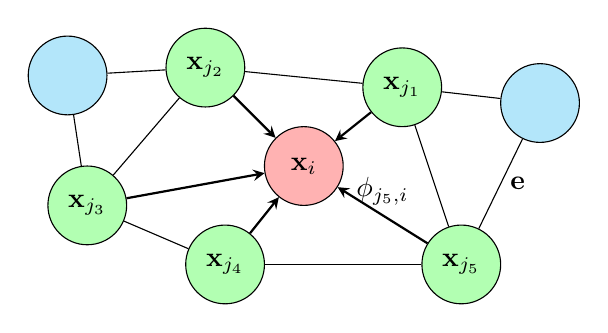
\begin{tikzpicture}[node distance=1.25cm]
        \node(main) [main_node] {$\mathbf{x}_i$};
        \node(neigh1) [neigh_node, right of=main, yshift=1cm] {$\mathbf{x}_{j_1}$};
        \node(neigh2) [neigh_node, left of=main, yshift=1.25cm] {$\mathbf{x}_{j_2}$};
        \node(neigh3) [neigh_node, left of=main, xshift=-1.5cm, yshift=-0.5cm] {$\mathbf{x}_{j_3}$};
        \node(neigh4) [neigh_node, below of=main, xshift=-1cm] {$\mathbf{x}_{j_4}$};
        \node(neigh5) [neigh_node, below of=main, xshift=2cm] {$\mathbf{x}_{j_5}$};

        \node(node1) [node, right of=neigh1, xshift=0.5cm, yshift=-0.2cm] {};
        \node(node2) [node, left of=neigh2, xshift=-0.5cm, yshift=-0.1cm] {};

        \draw[arrow] (neigh1) -- (main);
        \draw[arrow] (neigh2) -- (main);
        \draw[arrow] (neigh3) -- (main);
        \draw[arrow] (neigh4) -- (main);
        \draw[arrow] (neigh5) -- node[above]{$\phi_{j_5, i}$} (main);

        \draw (neigh1) -- (neigh2);
        \draw (neigh1) -- (neigh5);
        \draw (neigh2) -- (neigh3);
        \draw (neigh3) -- (neigh4);
        \draw (neigh4) -- (neigh5);
        \draw (neigh1) -- (node1);
        \draw (neigh5) -- node[right]{$\mathbf{e}$} (node1);
        \draw (neigh2) -- (node2);
        \draw (neigh3) -- (node2);
    \end{tikzpicture}
    \caption{Illustration of the message passing scheme}
\end{figure}

Different graph neural networks architecture can be constructed by specifying all this functions, in
particular the update function, since aggregation operation usually is chosen from the fixed list of
functions such as $\min$, $\max$, mean, sum, product, etc.

Also it is worth to point out, that the graph neural network has a property of locality: the next state of the node depends only on
the current state of the adjacent nodes (and incident edges if they exist), therefore the receptive field
of every node is limited to the number of layers or number of applying the layer to the given graph (usually
on each step different layers are applied).

\subsection{Minimum cost multicut problem}

The minimum cost multicut problem is a combinatorial problem which consists in binary
edge labeling for a given, not necessarily complete, weighted graph. The resulted labeling induced
a partitioning of the graph and can be recognized as an analogue of an instance segmentation for graphs and
that's why has a lot real-world application in computer vision and other fields.

\begin{definition}
    Let $G = (V, E, w)$ be a connected weighted graph, where $V$ is a set of nodes, $E$ -- set of edges and
    $w: E \to \mathbb{R}$ is a weight/cost function. Then the minimum cost multicut
    problem\footnote{The original paper has a typo in the definition of the problem}
    is the following:

    \begin{alignat}{2}
        \min_{y \in \{0, 1\}^E} \quad &
        c(y) = \sum\limits_{e \in E} w_e y_e                                                      \label{def:cost}                  \\
        \text{subject to:}      \quad &
        y_e \leq \sum\limits_{e' \in C \setminus \{e\}} y_{e'}                                         \label{def:cycle_constraint} \\
                                      & \forall C \in \text{cycles}(G), \forall e \in C \nonumber
    \end{alignat}
\end{definition}

The label $1$ means that the corresponding edge is cut.
And the cycle constraints ensure that if the edge was cut then there is no other path in the graph which connects
incident nodes of this edges.

This constraints can be reduced to only chordless cycles as it was shown by \citet{chopra1993partition}, but still for the
non complete graphs (where triangles inequality is sufficient) the constraints grows with size of graph exponentially, so can be
their enumeration can be practically infeasible.

From the point of view of hardness of this integer linear programming problem it is worth to mention that minimum cost multicut
is NP-hard.


\section{Problem statement}

In their article \citet{jung2022learning} address the problem of applying graph neural networks to
the minimum cost multicut problem in order to optimize runtime, but with preserving an
accuracy (in terms of cost) of the solution. And since every neural network consists of
data, architecture, loss function and training process, answering these question is one of the main
task of the paper as well.

\section{Conceptual contributions}

\subsection{General pipeline}

The main conceptual contribution of the paper is a pipeline of applying the graph neural network to
the instance of minimum multicut problem defining by graph. This pipeline can be expressed in the following way.

\begin{algorithm}[h]
    \SetKwInOut{Input}{Input}
    \caption{GNN multicut pipeline}\label{alg:pipeline}
    \Input{$G = (V, E, w)$ -- graph}
    \KwResult{$y \in \{ 0, 1 \}^E$ -- binary labeling of the edges}

    \ForEach{$i \in V$}
    {
        $
            \mathbf{x}_i \gets \left(
            \sum\limits_{j \in \mathcal{N}^{+}(i)} w_{ij},
            \sum\limits_{j \in \mathcal{N}^{-}(i)} w_{ij}
            \right)
        $ \;
        $\mathbf{h_i} \gets \text{GNN}(\mathbf{x_i})$ \;
    }
    \ForEach{$e_{ij} \in E$}
    {
        $y_{ij} \gets \frac{1}{2} \left( \text{MLP} \left( \substack{\mathbf{h_i} \\ \mathbf{h_j}} \right) +
            \text{MLP} \left( \substack{\mathbf{h_j} \\ \mathbf{h_i}} \right) \right) > 0.5$ \;
    }
    Enforce cycle consistency via message passing
\end{algorithm}

Generally, the idea of the approach can be expressed as transforming of the problem of graph partitioning into the real
value clustering problem of node's embeddings, which can be solved by a various methods: in this case with use of MLP.
Then, edges which are incident to the nodes which belong to the different clusters should be cut and
edges which corresponds to the nodes of the same cluster should be preserved.

To perform this transformation from graph to real value node's embeddings an instance of the graph neural
network is being used.

In order to perform the calculation of node embeddings by the message passing approach the input of
graph neural network has to contain initial node features. But since an instance of the minimum cost multicut problem
has only the edge weights authors have proposed the method of computing these features: for each node
they provide 2 dimensional vector where the first component is the sum of all positive incident edge weights and
the second component -- sum of all negative incident edge weights.

Then high dimensional node's embeddings is computed by applying a graph neural network, which will be
discussed in details in the next subsection. The main point to highlight in this regard is that
message passing step  can be run for every node in parallel on GPU which significantly improve runtime of the
full pipeline and which is easy to implement because of existence of a lot deep learning libraries
which provide GPU acceleration out of the box.

On the next step edge classification is performed with use of MLP, i.e. the node's embeddings $\mathbf{h_i}$ and
$\mathbf{h_j}$ of the incident edge $ij$ stacked together in two vectors
$\left( \substack{\mathbf{h_j} \\ \mathbf{h_i}} \right)$ and
$\left( \substack{\mathbf{h_i} \\ \mathbf{h_j}} \right)$. The mean of the MLP with sigmoid head
output is used as a confidence whether an edge should be cut. The final prediction computed by thresholding
this value at $0.5$.

MLP based edge classification requires two vectors because the input graph is considered to be undirected and
MLP is not permutation invariant: the order of inputs
matter. Also the averaging of the MLP outputs is not so expressible and reliable way to compute the labeling.
The ideas of how to improve this step will be discussed in section \ref{sec:ortho_emb}.

The computed solution can be infeasible since there is no guarantee that cycle consistency \eqref{def:cycle_constraint} won't be
violated. That's why the postprocessing step is required. This step consists in rounding (uncuting wrongly cut edges) of the computed
labeling to enforce the feasibility of the solution. It can be computed by a message passing approach, but since
neither source code nor detailed explanation has been provided by authors we propose our own algorithm \ref{alg:postprocessing}.

\begin{algorithm}[h]
    \SetKwInOut{Input}{Input}
    \caption{Cycle consistency enforcing} \label{alg:postprocessing}
    \Input{$G = (V, E, w)$ -- graph, $y \in \{ 0, 1 \}^E$ -- binary labeling of the edges}
    \KwResult{$\hat{y} \in \{ 0, 1 \}^E$ -- feasible solution}

    \For{$i \in \{1, \dots, |V| \}$}
    {
        $c_i = i$ \Comment{initial class label}
    }

    \For{$n \in \{ 1, \dots, \text{diag}(G) \}$}
    {
        $c \gets \text{MPN}(c)$ \Comment{update rule \eqref{def:postprocessing_mpn}}
    }

    \ForEach{$e_{ij} \in E$}
    {
        $\hat{y}_{ij} \gets c_i = c_j$ \;
    }

\end{algorithm}

For the given graph on the first step for every node we assign different labels which means
that we start with totally separated clusters where only 1 node belong to every particular cluster.
This labels is used as a node's features in the following step.

\begin{figure*}[h]
    \centering
    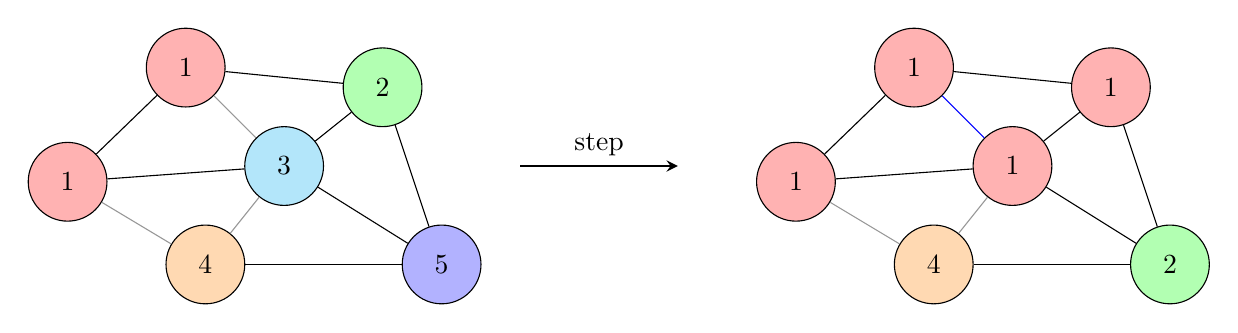
\begin{tikzpicture}[node distance=1.25cm]
        \node(root) [node] {3};
        \node(node1) [node, fill=green!30, right of=root, yshift=1cm] {2};
        \node(node2) [node, fill=red!30, left of=root, yshift=1.25cm] {1};
        \node(node3) [node, fill=red!30, left of=root, xshift=-1.5cm, yshift=-0.2cm] {1};
        \node(node4) [node, fill=orange!30, below of=root, xshift=-1cm] {4};
        \node(node5) [node, fill=blue!30, below of=root, xshift=2cm] {5};

        \node(root2) [node, fill=red!30, right of=root, xshift=8cm] {1};
        \node(node21) [node, fill=red!30, right of=root2, yshift=1cm] {1};
        \node(node22) [node, fill=red!30, left of=root2, yshift=1.25cm] {1};
        \node(node23) [node, fill=red!30, left of=root2, xshift=-1.5cm, yshift=-0.2cm] {1};
        \node(node24) [node, fill=orange!30, below of=root2, xshift=-1cm] {4};
        \node(node25) [node, fill=green!30, below of=root2, xshift=2cm] {2};

        \draw (node1) -- (root);
        \draw[color=gray!80] (node2) -- (root);
        \draw (node3) -- (root);
        \draw[color=gray!80] (node4) -- (root);
        \draw (node5) -- (root);

        \draw (node1) -- (node2);
        \draw (node1) -- (node5);
        \draw (node2) -- (node3);
        \draw[color=gray!80] (node3) -- (node4);
        \draw (node4) -- (node5);

        \draw[arrow] (3, 0) -- node[above]{step} (5, 0);

        \draw (node21) -- (root2);
        \draw[color=blue] (node22) -- (root2);
        \draw (node23) -- (root2);
        \draw[color=gray!80] (node24) -- (root2);
        \draw (node25) -- (root2);

        \draw (node21) -- (node22);
        \draw (node21) -- (node25);
        \draw (node22) -- (node23);
        \draw[color=gray!80] (node23) -- (node24);
        \draw (node24) -- (node25);
    \end{tikzpicture}
    \caption{Illustration of the step of the message passing postprocessing network: colors and labels in nodes corresponds to the
        cluster of nodes: same color and label -- same cluster. Black edges is a uncut edges of the original graph $G$ and
        \textcolor{gray!80}{gray} -- cut edges of $G$. After a message passing step 3 nodes which have been connected by uncut edges
        changed their labels to the minimal label among the neighborhood. At the same time the node with label 4 didn't changed their label
        because it is not connected by uncut edge to any node with smaller label on this step. Also we denote with \textcolor{blue}{blue} color edge that became
        incident to nodes from the same cluster and therefore
        on the last step of postprocessing algorithm will be restored.} \label{fig:postprocessing}
\end{figure*}

The key component of the postprocessing step is an message passing rule, which is the following:
\begin{equation} \label{def:postprocessing_mpn}
    c_i^{t+1} = \min \left\{ c_i^{t}, \min\limits_{j \in i \cup \mathcal{N}(i)} \left\{ (1 - y_{ij})c_j^{t} + y_{ij} \cdot \infty \right\}  \right\}
\end{equation}
This message passing network on every their step relabel nodes in a way that the resulted label is
equal to the minimum label among the node itself and their adjacent nodes unless adjacent node has been cut.
So, this step is just some variation of a connected component algorithm. But since it is implemented as a message passing
manner it can be parallelized on GPU in the same way as a GNN. But to be sure that we complete finding
all components (merge every component which should be merged for the worst case: linked list) message passing
relabeling has to be run number of steps which is equal to diameter of a given graph (but in real application can
be bounded by a relatively large number or computed precisely if the structure of graph (e.g. grid graph)
is known). The example of the step of a message passing network is given on figure \ref{fig:postprocessing}

The last step of postprocessing algorithm is responsible for uncut wrongly cut edges by restoring edges
which belongs to the same cluster (that means that there is a path in graph made by uncut edges which
connect this two nodes and therefore constraints \eqref{def:cycle_constraint} have been violated).


\subsection{Graph neural network architectures}

\subsection{Loss function}

\subsection{Training process and datasets}

\section{Empirical contributions (if any, max.~1 column)}

\emph{State briefly the main empirical findings of the article(s) you are summarizing (if any).
    Do not copy or reproduce any figures or tables.}

\section{Ideas to improve the discussed approach}
\subsection{Orthogonal embeddings} \label{sec:ortho_emb}
\subsection{Relaxed Cycle Consistency Loss}
\subsection{Edge Weight Embedding}

\subsection{Unsupervised formulation}
\subsection{Self-prior learning / finetuning}

\bibliography{../references.bib}
\bibliographystyle{plainnat}

\end{document}

